% ======================================================================
%  PAC-Former: backbone + four MI-operator variants (v1 / v2 / v3 / v4)
%  Compile:  pdflatex mi_architectures.tex
%  (needs TikZ; uses only standard libraries -> compiles out of the box)
%
%  Colour legend:
%    blue  = learnable module (Linear / Conv / projection)
%    gray  = parameter-free op (reshape, mean, softmax, matmul, concat)
%    orange= PAC prior path  (Hilbert, MVL coupling, pac_scale)  <-- our novelty
%    green = gating (v4 only)
% ======================================================================
\documentclass[border=8pt]{standalone}
\usepackage{tikz}
\usepackage{amsmath}
\usetikzlibrary{positioning,arrows.meta,calc,fit,backgrounds}

\tikzset{
  box/.style   ={draw, rounded corners=2pt, minimum height=7mm,
                 minimum width=22mm, align=center, font=\footnotesize, thick},
  learn/.style ={box, fill=blue!12,  draw=blue!60},
  op/.style    ={box, fill=black!6,  draw=black!45},
  pac/.style   ={box, fill=orange!18,draw=orange!80},
  gate/.style  ={box, fill=green!16, draw=green!60},
  io/.style    ={box, fill=black!4,  draw=black!75, minimum width=30mm},
  add/.style   ={circle, draw, thick, inner sep=0pt, minimum size=5.5mm, font=\small},
  fl/.style    ={-{Stealth[length=2.4mm]}, thick},
  shp/.style   ={font=\scriptsize\ttfamily, midway, fill=white, inner sep=1pt},
  grp/.style   ={draw, dashed, rounded corners=3pt, inner sep=5pt}
}
\newcommand{\nb}{n_b}

\begin{document}

% ======================================================================
% FIGURE 0 -- overall PAC-Former backbone (the mixer is the swappable slot)
% ======================================================================
\begin{tikzpicture}[node distance=6mm]
  \node[io]                     (raw)  {Raw EEG \; $(B,C,T)$};
  \node[op, below=of raw]       (aug)  {RandomAugment};
  \node[learn, below=of aug]    (sinc) {Sinc bandpass bank\\$\to (B,C,\nb,T)$};

  % two branches out of sinc
  \node[learn, below left=8mm and 4mm of sinc]  (conv)
        {per-band Conv1d\\(patch tokenizer)};
  \node[pac,   below right=8mm and 4mm of sinc] (hilb)
        {Hilbert $\to \varphi,\,A$\\$(B,C,\nb,T)$};

  \node[op, below=14mm of sinc] (tok)  {tokens $(B,\nb P,D)$};

  \node[draw, dashed, rounded corners=3pt, fill=blue!4,
        minimum width=52mm, minimum height=20mm, below=9mm of tok] (blk) {};
  \node[font=\footnotesize\bfseries, above=0.5mm of blk.north] {Encoder block $\times L$};
  \node[op,   at=($(blk.center)+(-14mm,4mm)$)] (ln1) {LayerNorm};
  \node[learn,fill=orange!18,draw=orange!80,
        at=($(blk.center)+(12mm,4mm)$)]        (mix) {\textbf{Mixer}\\(swappable)};
  \node[op,   at=($(blk.center)+(-14mm,-5mm)$)] (ln2) {LayerNorm};
  \node[learn,at=($(blk.center)+(12mm,-5mm)$)]  (ffn) {FFN};

  \node[learn, below=10mm of blk] (head) {Pool + Head};
  \node[io, below=of head]        (out)  {logits $(B,\,\text{n\_cls})$};

  \draw[fl] (raw)--(aug);
  \draw[fl] (aug)--(sinc);
  \draw[fl] (sinc)--(conv);
  \draw[fl] (sinc)--(hilb);
  \draw[fl] (conv)--(tok);
  \draw[fl] (tok)--(blk);
  \draw[fl] (blk)--(head);
  \draw[fl] (head)--(out);
  % phase/amp routed into the mixer
  \draw[fl,orange!80,dashed] (hilb.east) to[out=0,in=0]
        node[shp,black]{$\varphi,A$} (mix.east);

  \node[font=\footnotesize, right=16mm of mix, text width=34mm, align=left]
        {The \textbf{Mixer} slot is where\\ attention / CoTAR / \textbf{MI (ours)}\\
         are swapped. The MI variants\\ (v1--v4) are detailed below.};
\end{tikzpicture}

% ======================================================================
% FIGURE 1 -- MI v1 : fixed PAC coupling used directly as softmax weights
%             (NO learned Q/K/V)
% ======================================================================
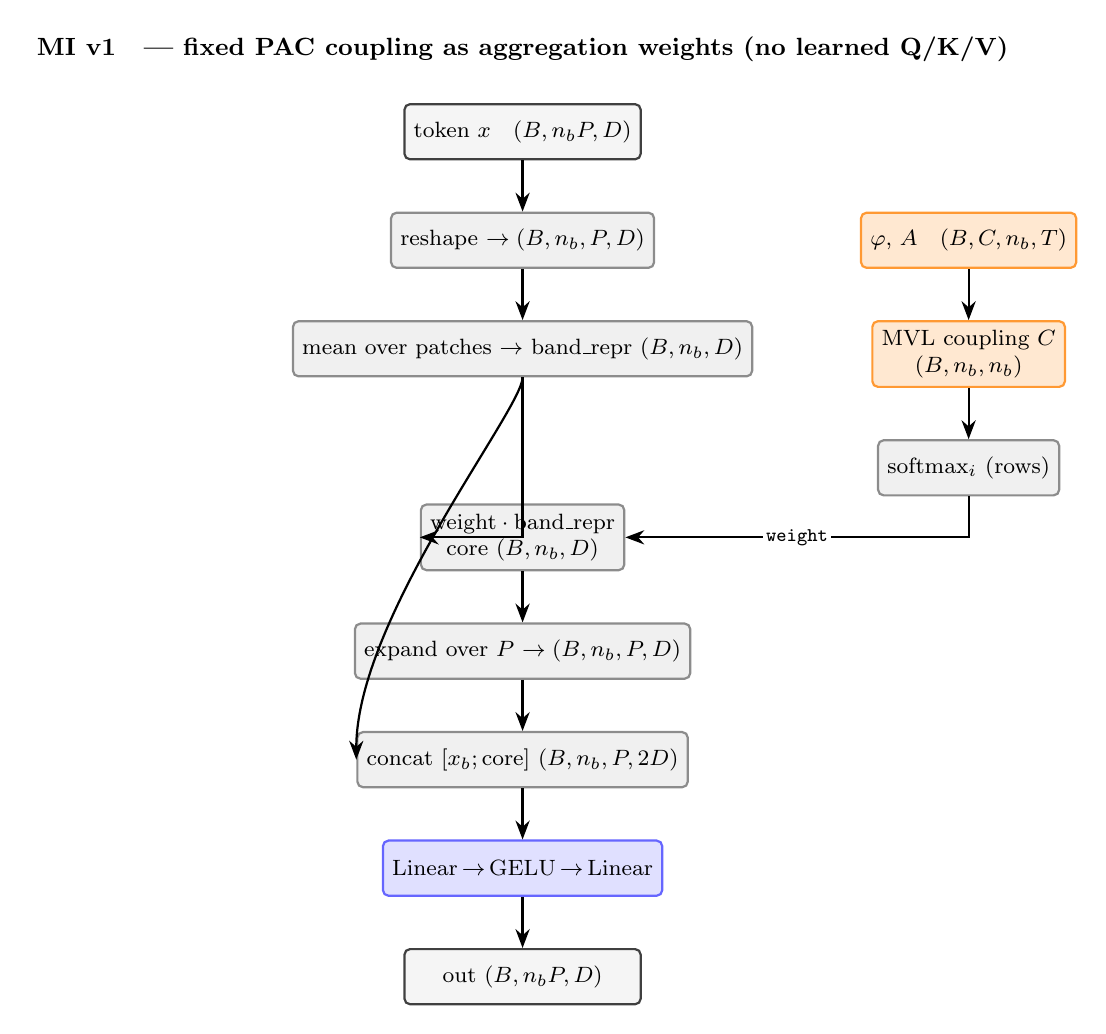
\begin{tikzpicture}[node distance=6.5mm]
  \node[font=\small\bfseries] (title) {MI v1 \; --- fixed PAC coupling as aggregation weights (no learned Q/K/V)};
  \node[io, below=4mm of title] (x) {token $x$ \; $(B,\nb P,D)$};
  \node[op, below=of x]  (rs)  {reshape $\to (B,\nb,P,D)$};
  \node[op, below=of rs] (mean){mean over patches $\to$ band\_repr $(B,\nb,D)$};

  % PAC branch (right)
  \node[pac, right=26mm of rs] (phi) {$\varphi,\,A$ \; $(B,C,\nb,T)$};
  \node[pac, below=of phi]     (coup){MVL coupling $C$\\$(B,\nb,\nb)$};
  \node[op,  below=of coup]    (sm)  {softmax$_i$ (rows)};

  \node[op, below=16mm of mean] (agg) {$\text{weight}\cdot\text{band\_repr}$\\core $(B,\nb,D)$};
  \node[op, below=of agg]  (exp) {expand over $P$ $\to (B,\nb,P,D)$};
  \node[op, below=of exp]  (cat) {concat $[x_b;\text{core}]$ $(B,\nb,P,2D)$};
  \node[learn, below=of cat](mlp) {Linear\,$\to$\,GELU\,$\to$\,Linear};
  \node[io, below=of mlp]  (out) {out $(B,\nb P,D)$};

  \draw[fl](x)--(rs); \draw[fl](rs)--(mean);
  \draw[fl](phi)--(coup); \draw[fl](coup)--(sm);
  \draw[fl](mean.south) |- (agg.west);
  \draw[fl](sm.south) |- (agg.east) node[shp,pos=0.75]{weight};
  \draw[fl](agg)--(exp);\draw[fl](exp)--(cat);
  \draw[fl](mean.south) .. controls +(0,-4mm) and +(0,18mm) .. (cat.west); % x_b skip
  \draw[fl](cat)--(mlp);\draw[fl](mlp)--(out);
\end{tikzpicture}

% ======================================================================
% FIGURE 2 -- MI v2 : PAC-biased cross-band attention, channel-MEAN coupling
% ======================================================================
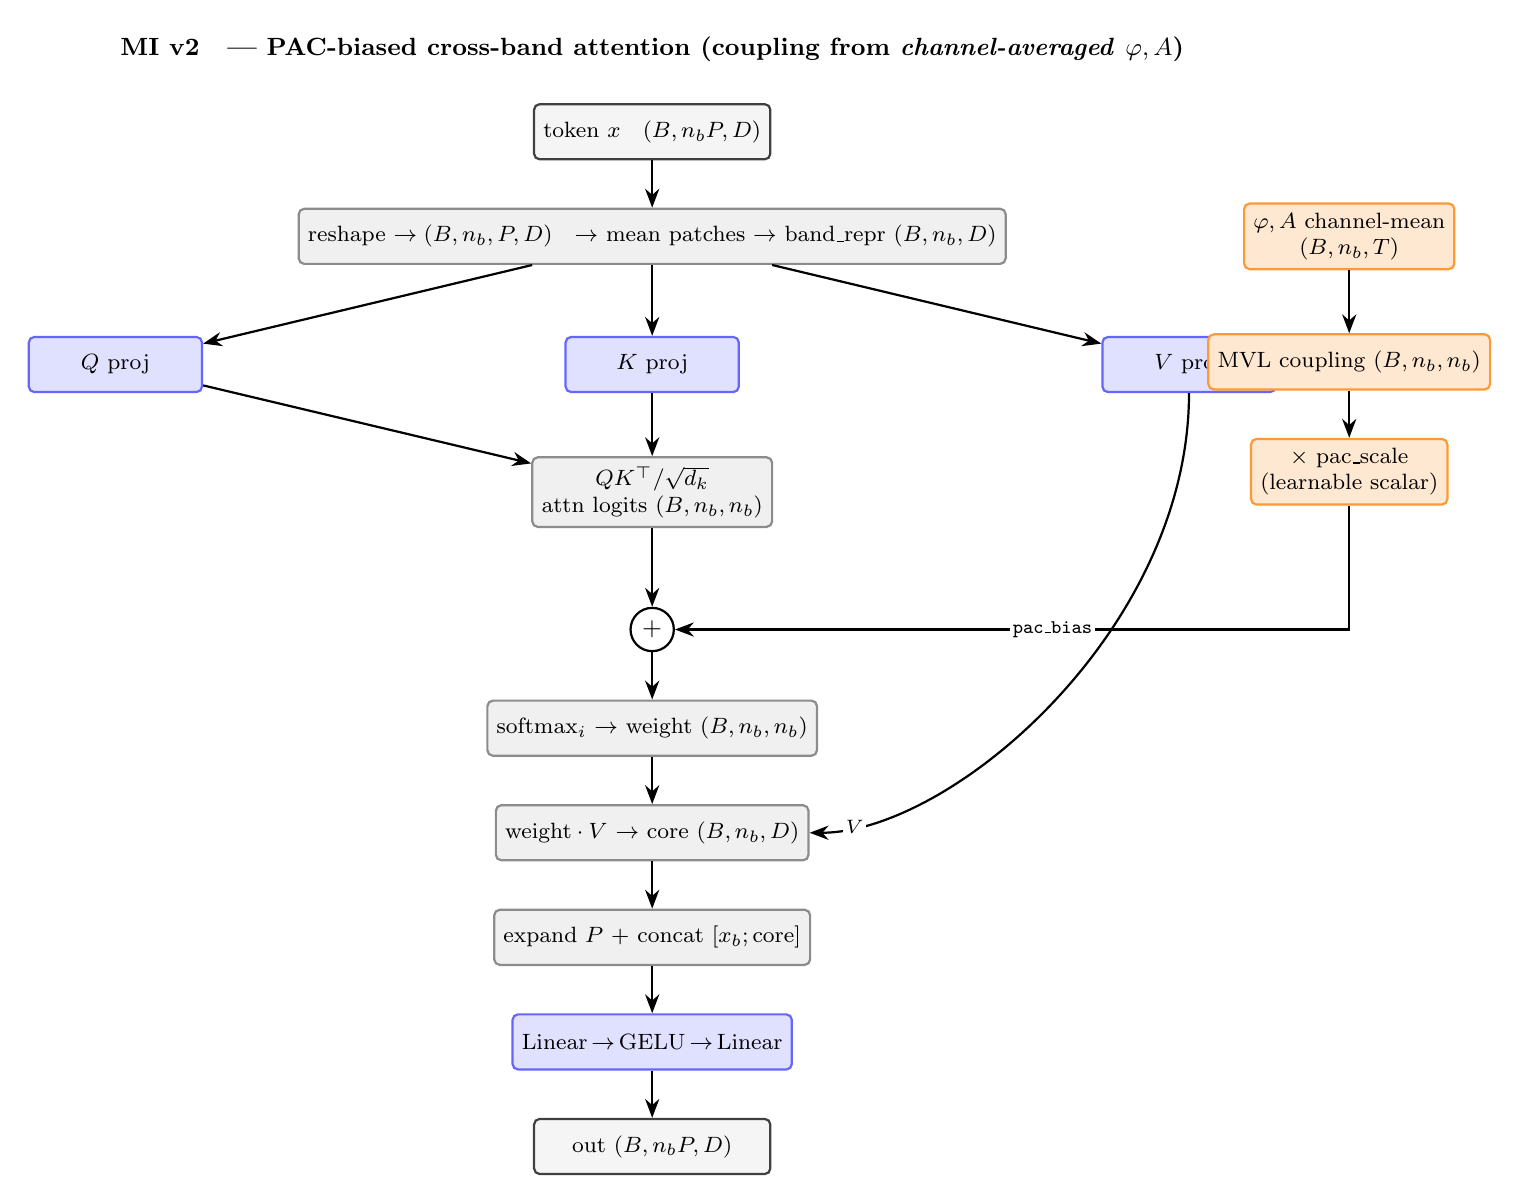
\begin{tikzpicture}[node distance=6mm]
  \node[font=\small\bfseries](title){MI v2 \; --- PAC-biased cross-band attention (coupling from \emph{channel-averaged} $\varphi,A$)};
  \node[io, below=4mm of title](x){token $x$ \; $(B,\nb P,D)$};
  \node[op, below=of x](rs){reshape $\to(B,\nb,P,D)$ \; $\to$ mean patches $\to$ band\_repr $(B,\nb,D)$};

  % learned Q/K/V
  \node[learn, below left=9mm and 12mm of rs](q){$Q$ proj};
  \node[learn, below=9mm of rs](k){$K$ proj};
  \node[learn, below right=9mm and 12mm of rs](v){$V$ proj};
  \node[op, below=8mm of k](qk){$QK^\top/\sqrt{d_k}$\\attn logits $(B,\nb,\nb)$};

  % PAC branch (right)
  \node[pac, right=30mm of rs](phi){$\varphi,A$ channel-mean\\$(B,\nb,T)$};
  \node[pac, below=8mm of phi](coup){MVL coupling $(B,\nb,\nb)$};
  \node[pac, below=of coup](ps){$\times\ \text{pac\_scale}$\\(learnable scalar)};

  \node[add, below=10mm of qk](add){$+$};
  \node[op, below=of add](sm){softmax$_i$ $\to$ weight $(B,\nb,\nb)$};
  \node[op, below=of sm](agg){$\text{weight}\cdot V$ $\to$ core $(B,\nb,D)$};
  \node[op, below=of agg](cat){expand $P$ + concat $[x_b;\text{core}]$};
  \node[learn, below=of cat](mlp){Linear\,$\to$\,GELU\,$\to$\,Linear};
  \node[io, below=of mlp](out){out $(B,\nb P,D)$};

  \draw[fl](x)--(rs);
  \draw[fl](rs)--(q);\draw[fl](rs)--(k);\draw[fl](rs)--(v);
  \draw[fl](q)--(qk);\draw[fl](k)--(qk);
  \draw[fl](phi)--(coup);\draw[fl](coup)--(ps);
  \draw[fl](qk)--(add);
  \draw[fl](ps.south) |- (add.east) node[shp,pos=0.72]{pac\_bias};
  \draw[fl](add)--(sm);\draw[fl](sm)--(agg);
  \draw[fl](v.south) .. controls +(0,-30mm) and +(18mm,0) .. (agg.east)
        node[shp,pos=0.9]{$V$};
  \draw[fl](agg)--(cat);\draw[fl](cat)--(mlp);\draw[fl](mlp)--(out);
\end{tikzpicture}

% ======================================================================
% FIGURE 3 -- MI v3 : same as v2 but PER-CHANNEL coupling  (<-- the winner)
% ======================================================================
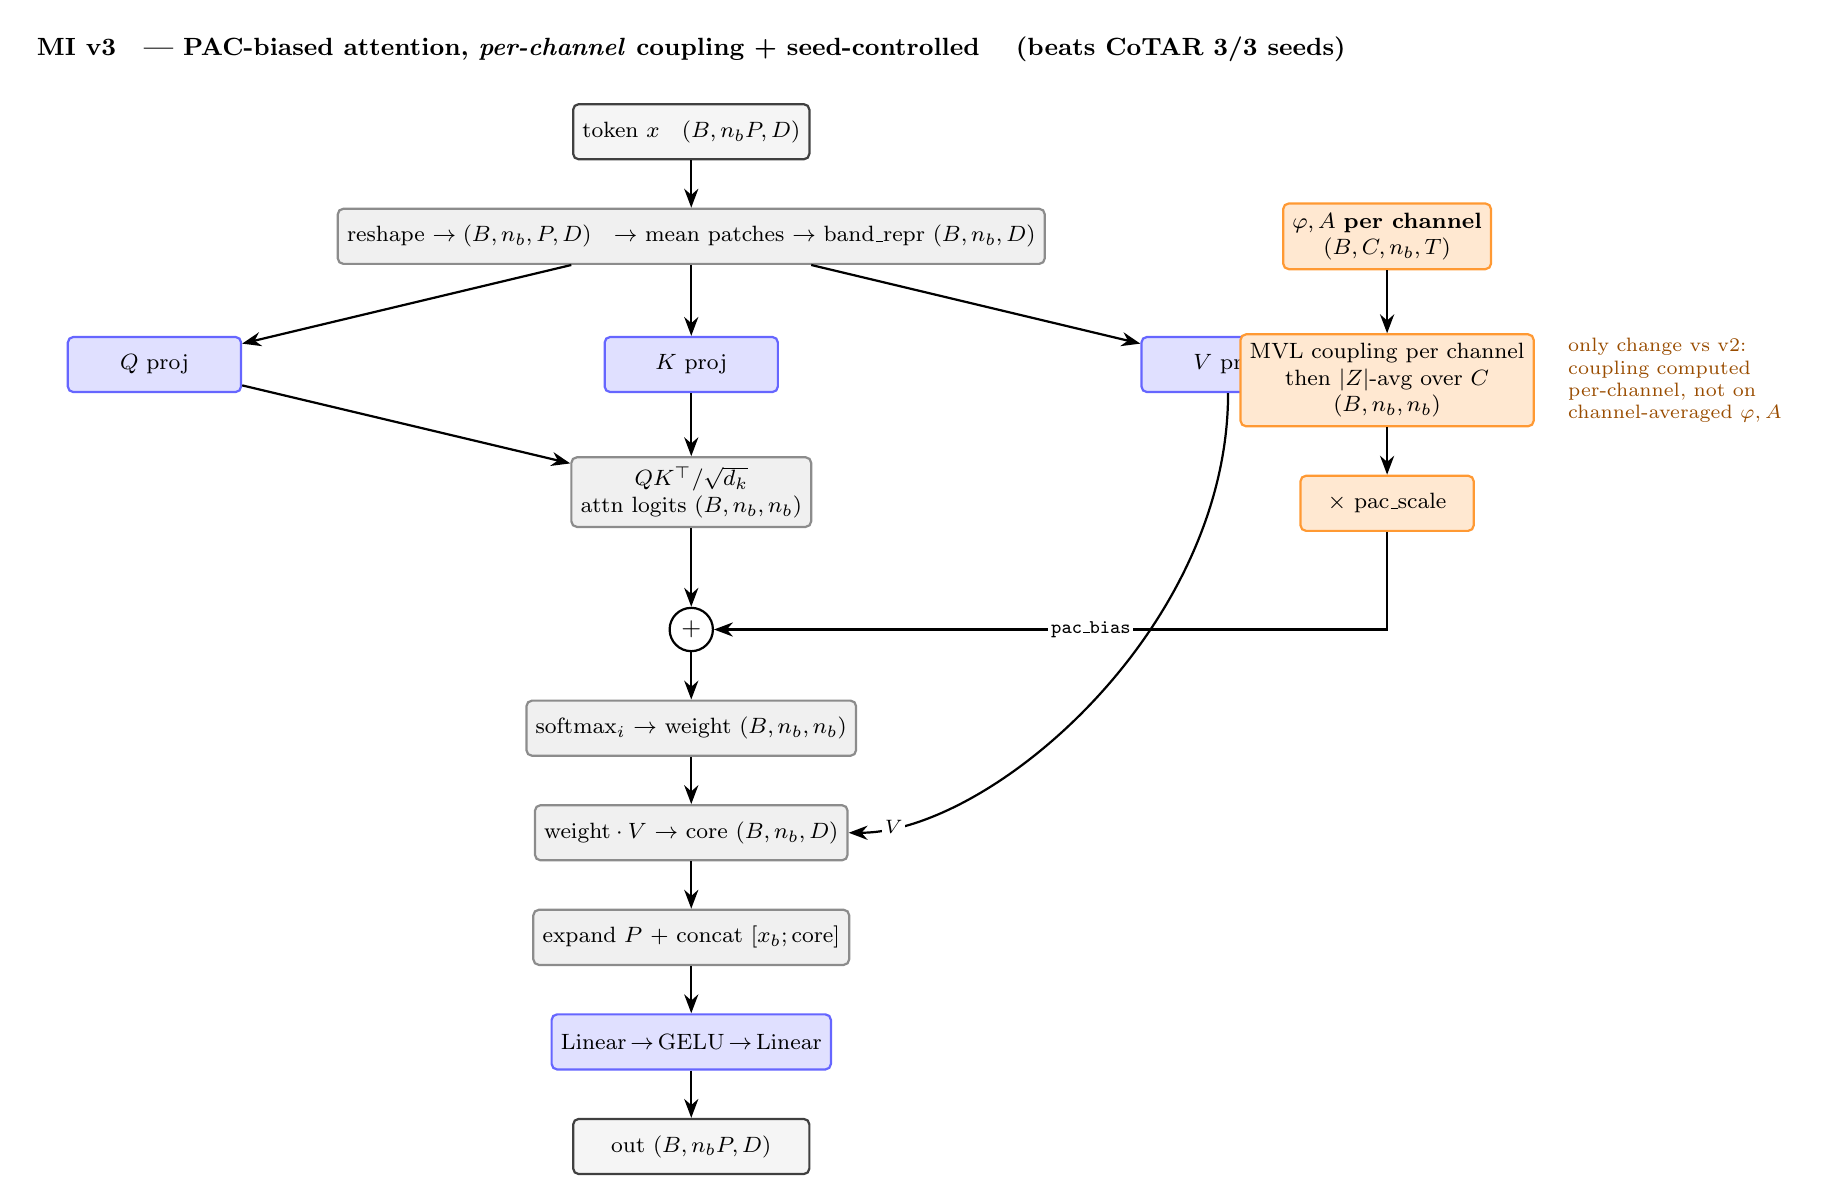
\begin{tikzpicture}[node distance=6mm]
  \node[font=\small\bfseries](title){MI v3 \; --- PAC-biased attention, \emph{per-channel} coupling + seed-controlled \;\; \textbf{(beats CoTAR 3/3 seeds)}};
  \node[io, below=4mm of title](x){token $x$ \; $(B,\nb P,D)$};
  \node[op, below=of x](rs){reshape $\to(B,\nb,P,D)$ \; $\to$ mean patches $\to$ band\_repr $(B,\nb,D)$};

  \node[learn, below left=9mm and 12mm of rs](q){$Q$ proj};
  \node[learn, below=9mm of rs](k){$K$ proj};
  \node[learn, below right=9mm and 12mm of rs](v){$V$ proj};
  \node[op, below=8mm of k](qk){$QK^\top/\sqrt{d_k}$\\attn logits $(B,\nb,\nb)$};

  % PAC branch -- the ONLY change vs v2 is this coupling box
  \node[pac, right=30mm of rs](phi){$\varphi,A$ \textbf{per channel}\\$(B,C,\nb,T)$};
  \node[pac, below=8mm of phi](coup){MVL coupling per channel\\then $|Z|$-avg over $C$\\$(B,\nb,\nb)$};
  \node[pac, below=of coup](ps){$\times\ \text{pac\_scale}$};

  \node[add, below=10mm of qk](add){$+$};
  \node[op, below=of add](sm){softmax$_i$ $\to$ weight $(B,\nb,\nb)$};
  \node[op, below=of sm](agg){$\text{weight}\cdot V$ $\to$ core $(B,\nb,D)$};
  \node[op, below=of agg](cat){expand $P$ + concat $[x_b;\text{core}]$};
  \node[learn, below=of cat](mlp){Linear\,$\to$\,GELU\,$\to$\,Linear};
  \node[io, below=of mlp](out){out $(B,\nb P,D)$};

  \draw[fl](x)--(rs);
  \draw[fl](rs)--(q);\draw[fl](rs)--(k);\draw[fl](rs)--(v);
  \draw[fl](q)--(qk);\draw[fl](k)--(qk);
  \draw[fl](phi)--(coup);\draw[fl](coup)--(ps);
  \draw[fl](qk)--(add);
  \draw[fl](ps.south) |- (add.east) node[shp,pos=0.72]{pac\_bias};
  \draw[fl](add)--(sm);\draw[fl](sm)--(agg);
  \draw[fl](v.south) .. controls +(0,-30mm) and +(18mm,0) .. (agg.east)
        node[shp,pos=0.9]{$V$};
  \draw[fl](agg)--(cat);\draw[fl](cat)--(mlp);\draw[fl](mlp)--(out);
  \node[font=\scriptsize, right=3mm of coup, text width=30mm, orange!60!black]
        {only change vs v2:\\ coupling computed\\ per-channel, not on\\ channel-averaged $\varphi,A$};
\end{tikzpicture}

% ======================================================================
% FIGURE 4 -- MI v4 : v3 + multi-head + per-head pac_scale + gated inject
%             (tried, no net gain, reverted)
% ======================================================================
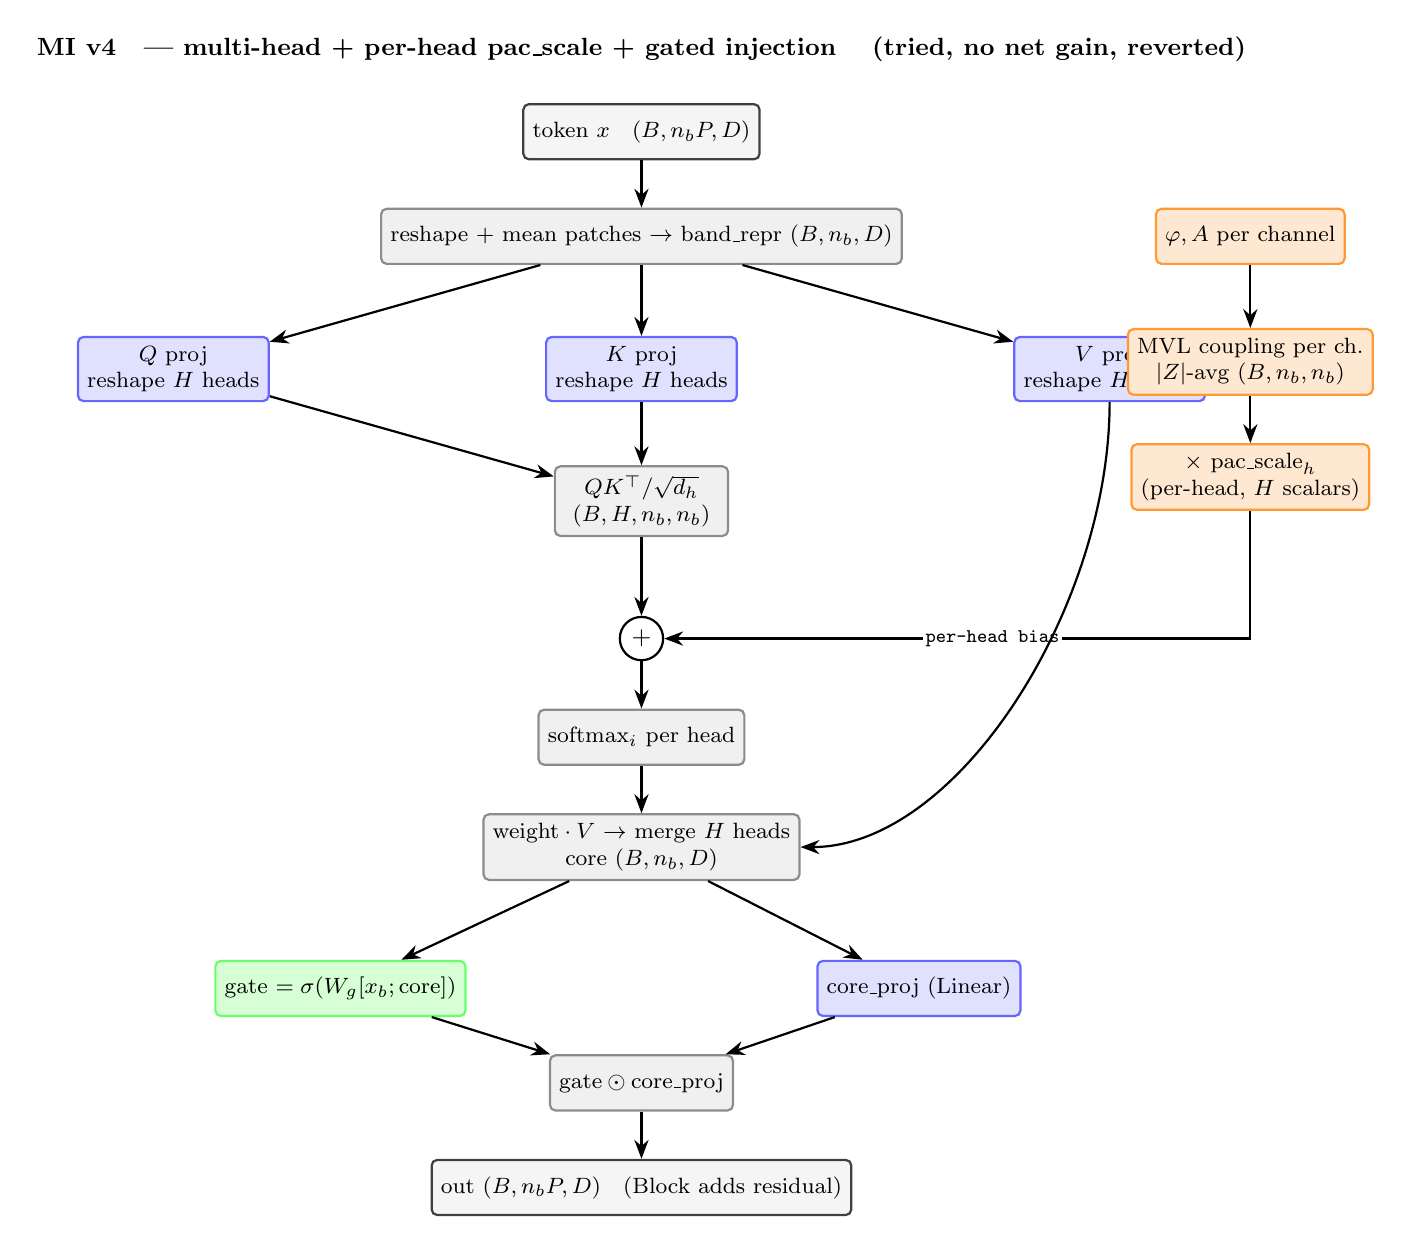
\begin{tikzpicture}[node distance=6mm]
  \node[font=\small\bfseries](title){MI v4 \; --- multi-head + per-head pac\_scale + gated injection \;\; (tried, no net gain, reverted)};
  \node[io, below=4mm of title](x){token $x$ \; $(B,\nb P,D)$};
  \node[op, below=of x](rs){reshape + mean patches $\to$ band\_repr $(B,\nb,D)$};

  \node[learn, below left=9mm and 14mm of rs](q){$Q$ proj\\reshape $H$ heads};
  \node[learn, below=9mm of rs](k){$K$ proj\\reshape $H$ heads};
  \node[learn, below right=9mm and 14mm of rs](v){$V$ proj\\reshape $H$ heads};
  \node[op, below=8mm of k](qk){$QK^\top/\sqrt{d_h}$\\$(B,H,\nb,\nb)$};

  \node[pac, right=32mm of rs](phi){$\varphi,A$ per channel};
  \node[pac, below=8mm of phi](coup){MVL coupling per ch.\\$|Z|$-avg $(B,\nb,\nb)$};
  \node[pac, below=of coup](ps){$\times\ \text{pac\_scale}_h$\\(per-head, $H$ scalars)};

  \node[add, below=10mm of qk](add){$+$};
  \node[op, below=of add](sm){softmax$_i$ per head};
  \node[op, below=of sm](agg){$\text{weight}\cdot V$ $\to$ merge $H$ heads\\core $(B,\nb,D)$};

  % gated injection
  \node[gate, below left=10mm and 2mm of agg](gate){gate $=\sigma(W_g[x_b;\text{core}])$};
  \node[learn, below right=10mm and 2mm of agg](cp){core\_proj (Linear)};
  \node[op, below=22mm of agg](mul){$\text{gate}\odot\text{core\_proj}$};
  \node[io, below=of mul](out){out $(B,\nb P,D)$ \; (Block adds residual)};

  \draw[fl](x)--(rs);
  \draw[fl](rs)--(q);\draw[fl](rs)--(k);\draw[fl](rs)--(v);
  \draw[fl](q)--(qk);\draw[fl](k)--(qk);
  \draw[fl](phi)--(coup);\draw[fl](coup)--(ps);
  \draw[fl](qk)--(add);
  \draw[fl](ps.south) |- (add.east) node[shp,pos=0.72]{per-head bias};
  \draw[fl](add)--(sm);\draw[fl](sm)--(agg);
  \draw[fl](v.south) .. controls +(0,-26mm) and +(20mm,0) .. (agg.east);
  \draw[fl](agg)--(gate);\draw[fl](agg)--(cp);
  \draw[fl](gate)--(mul);\draw[fl](cp)--(mul);
  \draw[fl](mul)--(out);
\end{tikzpicture}

\end{document}
